\documentclass[10pt]{article}

\usepackage{amsmath}
\usepackage{amssymb}
\usepackage{tabu}
\usepackage{lmodern}
\usepackage{graphicx}
\usepackage[space]{grffile}
\usepackage{subfigure}
\usepackage{longtable}
\usepackage{multirow}
\usepackage[margin=1.0in]{geometry}
\renewcommand{\baselinestretch}{2.0}

%\usepackage[font=small,labelfont=bf,labelsep=period]{caption}
\usepackage[style=authoryear,sorting=nyt,url=false,isbn=false,doi=false,firstinits=true,backend=biber]{biblatex}

\renewcommand{\baselinestretch}{2.0}
\renewcommand*\contentsname{Table of Contents}
%\captionsetup{font={stretch=2.0}}

\DeclareNameAlias{default}{last-first}

\DefineBibliographyStrings{english}{%
	andothers = {\addcomma\addspace\textsc{et\addabbrvspace al}\adddot},
	and = {\textsc{and}}
}
\renewcommand*{\labelnamepunct}{\space\space}

\renewbibmacro{in:}
{%
	\ifentrytype{article}{%
	}{%
		\printtext{\bibstring{in}\intitlepunct}%
	}%
}
\renewbibmacro*{volume+number}{%
	\printfield{volume}%
	\setunit*{\addcomma\space}%
	\printfield{number}%
	\setunit{\addcomma\space}}

\DeclareFieldFormat{pages}{#1}

\renewbibmacro*{publisher+location+date}{%
	\printlist{publisher}%
	\setunit*{\addcomma\space}%
	\printlist{location}%
	\setunit*{\addcomma\space}%
	\usebibmacro{date}%
	\newunit}

\renewcommand{\newunitpunct}{\addcomma\space}
\DeclareFieldFormat[article,inbook,incollection,inproceedings,patent,thesis,unpublished]{title}{#1} 
\DeclareFieldFormat{year}{#1} 

\addbibresource{refs/ident_refs.bib}

\begin{document}
\paragraph{Outline:}
\begin{itemize}
	\item Importance of parameter values for estimating in vivo response using kinetic models of metabolism and consequently for metabolic network design using kinetic models of metabolism
	\item The need for parameter identifiability to determine unique and true parameter values from observed data
	\item Types and purpose of identifiability for parameters
	\item Methods for structural identifiability and existing methods for practical identifiability
	\item Lack of methods for practical identifiability and consequently experimental design (not covered?)
	\item work done in this paper for practical identifiability			
	\item scalability of computer algebra-based methods for structural identifiability (using CRNT to reduce networks to make structural identifiability scalable) (move to discussion - may be in discussion)
\end{itemize}
\section{Introduction:}
Kinetic models of metabolism can be used to study the dynamic characteristics of metabolic networks. In these models, ordinary differential equations (ode) are used to express the rate of change of metabolite concentrations ($x$) as a function of the reaction fluxes ($v$) in the metabolic network (Equation \ref{eq:kinstoich}). The matrix $\mathbf{S}$ in Equation (\ref{eq:kinstoich}a) defines the stoichiometric relationship between the fluxes and the concentrations of the metabolic network.
\begin{subequations}\label{eq:kinstoich}
	\begin{align}
	\dot{x} = \mathbf{S}v\\
	v = f(x, \theta, u)
	\end{align}
\end{subequations}
The expression for the nonlinear function ($f$) used to describe each reaction flux $v_i$ in a kinetic model (Equation \ref{eq:kinstoich}b) is dependent on the enzyme kinetic mechanism that is used to model the reaction \parencite{Heijnen2005, Link2014, Machado2011, Srinivasan2015}. Accordingly, $f$ is a nonlinear function of the metabolite concentrations, enzyme kinetic parameters ($\theta$) and other input concentrations ($u$). 

The ability to predict the steady state and dynamic responses of metabolic networks, under in vivo conditions, to different perturbations is dependent on the numerical values of the enzyme kinetic parameter values ($\theta$) in Equation (\ref{eq:kinstoich}). Analyzing the ability of a metabolic network to exhibit dynamic characteristics like multiple steady states and oscillations, irrespective of the structure of the network, is one example where parameter values might play a crucial role \parencite{Srinivasan2015, Vital-Lopez2006}(Srinivasan et al., 2017?). The use of in vitro, or unreliable in vivo parameter estimates, reduces confidence in the model predicted behaviour. Consequently, the reduction in confidence hampers the use of these models to gain insight into the functioning of metabolic networks \parencite{Tran2008, Chakrabarti2013a}. The insights gained from the use of kinetic models are subsequently used to design changes to these metabolic networks to achieve various goals. These goals could either be to increase metabolite production for biosynthesis of different chemicals \parencite{Almquist2014, Khodayari2016, Costa2016, Andreozzi2016}(Srinivasan et al., 2017) or to find therapeutic targets to cure ailments \parencite{Apaolaza2017}. Hence, an increase in uncertainty in model predicted responses is also an obstacle for using the predicted responses as a basis for designing the metabolic networks to achieve these goals.  

If all intracellular metabolite concentrations can be measured over a time course, a nonlinear programming problem can be formulated to estimate the enzyme kinetic parameters ($\theta$) in Equation (\ref{eq:kinstoich}), based on the measured data. The minimization of least square error between the measured ($x^*$) and modeled ($x$) concentrations, weighted by the variance in the experimental data $\sigma_{kl}^*$ for each concentration at each time point, is used as an objective function (Equation \ref{eq:lsqopt}a) for the optimization problem (Equation \ref{eq:lsqopt}). The parameter values are determined within fixed upper ($\theta_u$) and lower ($\theta_l$) bounds (Equation \ref{eq:lsqopt}b). 
\begin{subequations}\label{eq:lsqopt}
	\begin{align}
	\underset{\theta}{\mathrm{min}} &\sum_{k=1}^{m}\sum_{l=1}^{d}\left(\frac{x_{kl}^*-x_{kl}}{\sigma_{kl}^*}\right)^2\\
	&\theta_l \le \theta \le \theta_u
	\end{align}
\end{subequations}

However, not all metabolite concentrations used in the model (Equation \ref{eq:kinstoich}) can be measured. Additionally, measurable fluxes in the metabolic network also need to be included as part of the parameter estimation problem. In such scenarios, the parameter estimation problem is modified to suit a new system of equations shown below (Equation \ref{eq:output}). The new system of equations is obtained by augmenting the original system (Equation \ref{eq:kinstoich}) with Equation (\ref{eq:output}c) that models the relationship between the measurable metabolite concentrations and fluxes ($y$) and the unmeasured concentrations ($x$) that are used in the original model (Equation \ref{eq:kinstoich}) above. The parameter vector ($\theta$) is augmented with additional parameters that define this relationship. These additional parameters also need to be estimated.
\begin{subequations}\label{eq:output}
	\begin{align}
	\dot{x} = \mathbf{S}v\\
	v = f(x, y, \theta, u)\\
	\dot{y} = h(x, y, \theta, u)
	\end{align}
\end{subequations}
In systems identification, the measured concentrations and fluxes ($y$) are called output or observed variables, and the unmeasured concentrations ($x$) are called the state variables. For estimating $\theta$, the metabolite concentrations $x$ in the optimization problem (Equation \ref{eq:lsqopt}) are substituted with the output variables $y$. 

However, the ability to determine unique solutions to parameters $\theta$ is governed by the identifiability of these parameters in the model \parencite{McLean2012}. The identifiability of parameters in nonlinear models can be classified into two categories: structural (or a priori) and practical (or posterior) identifiability. 	
Any system (Equation \ref{eq:output}) is said to be structurally identifiable if, for an input-output mapping defined by $y = \Phi(\theta,u)$ for at least one input function $u$, any two values of parameters $\theta_1$ and $\theta_2$ satisfy the relationship in Equation (\ref{eq:stident}) below.
\begin{align}\label{eq:stident}
\Phi(\theta_1,u) = \Phi(\theta_2,u) \iff \theta_1 = \theta_2
\end{align}
Accordingly, the system can have a unique solution, a finite number of non-unique solutions or an infinite number of solutions for all input functions, and is said to be structurally globally identifiable, locally identifiable or non-identifiable, respectively. So, the structural identifiability of parameters in a dynamic model helps establish the presence or absence of a relationship between the unobservable state variables and the observable output variables. Consequently, the effect of model structure and parameterization on the ability to infer true parameter values from experimental data is determined by the structural identifiability of the parameter. 

Experimental data from many physical systems is usually noisy, and when parameters are estimated on the basis of noisy data, the ability to estimate unique parameter values to satisfy Equation (\ref{eq:stident}) is referred to as practical identifiability. So, the effect of the available experimental data on the ability to estimate unique parameter values is determined by the practical identifiability of the parameter. Accordingly, practical identifiability of a parameter is contingent upon the nature, quality and quantity of data available to estimate the parameter as opposed to the structure and parameterization of the model. 

Thus, on the one hand, establishing the structural identifiability of parameters enables one to propose models that are not only appropriate representations of physical processes, but also are parameterized in such a way that the value of these parameters can be estimated from measurable data. On the other hand, establishing practical identifiability of parameters in any model helps design experiments that are minimal, informative and useful for parameter estimation.

Methods and tools for structural identification of parameters based on differential algebra \parencite{Ljung1994, Audoly2001, Bellu2007} and profile likelihood \parencite{Raue2009a} are available. However, only the profile likelihood-based methods enable experimental design by facilitating practical identification of parameters. Nonetheless, this method still depend on solving a non-convex nonlinear least squares problem (Equation \ref{eq:lsqopt}) to get likelihood estimates of parameters, and hence still suffers from all the inherent difficulties associated with obtaining global optimal solutions for non-convex optimization problems. This also makes it un-scalable for experimental design and practical identifiability of parameters in kinetic models of large metabolic networks.

In this paper, we propose a scalable methodology to establish practical identifiability for parameters in kinetic models of metabolism using abundantly available steady state concentration and flux data. We present a computer algebra-based method that can facilitate experimental design through practical identifiability of parameters separately for each individual reaction within a metabolic network based on available steady state experimental data. We illustrate the utility of this method by applying it to a small network of gluconeogenesis in \textit{E. coli} and demonstrating our ability to propose experiments that will facilitate parameter estimation for a kinetic model of this network. We also demonstrate the scalability of the proposed methodology to facilitate experimental design by applying it to a relatively larger metabolic network of the human red blood cell hepatocyte. 	

\section{Methods:}	
\begin{figure}[!tbhp]
	\centering{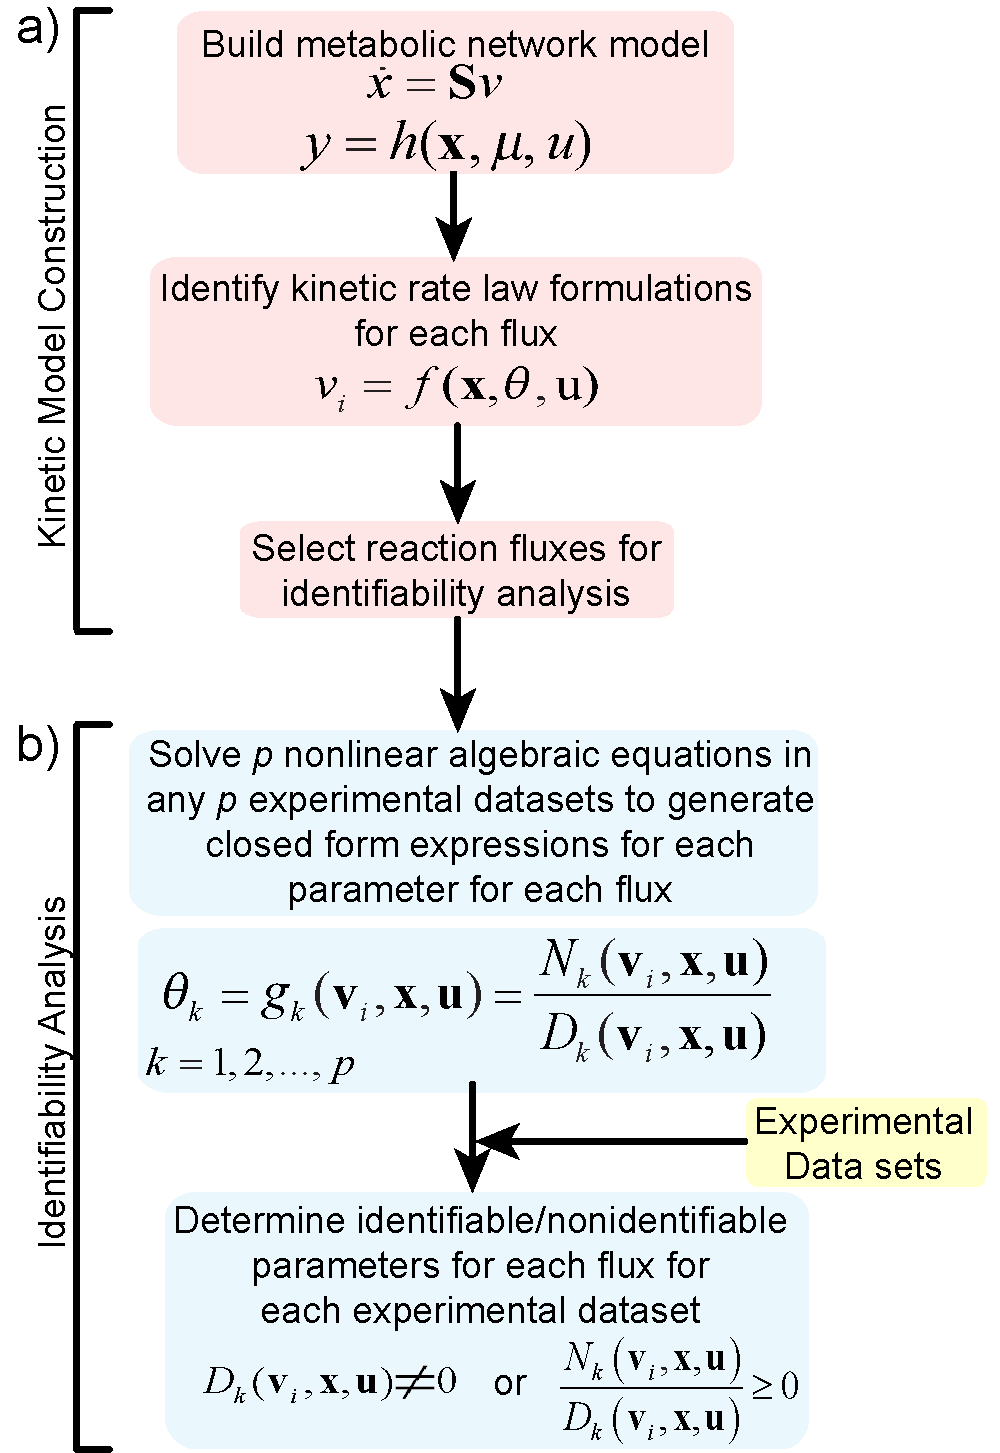
\includegraphics[width=.6\textwidth,height=.6\textheight,keepaspectratio]{C:/Users/shyam/Documents/Courses/CHE1125Project/Results/ident/figure3/ident_analysis}}
	\caption{A flow diagram showing the methodology developed to establish practical identifiability of parameters in kinetic models of metabolism. a) The steps for the construction of a kinetic model of a metabolic network are shown. The choice of rate law formulations to describe metabolic fluxes influences the identification methodology. The identifiability of parameters for each flux can be established independently. b) The steps for identifiability analysis for parameters of a single flux are shown.}\label{fig:ident-flowchart}
\end{figure}	
\subsection{A method for practical identifiability of kinetic models of metabolism:}\label{sec:ident}
In this section, we show how practical identifiability of kinetic parameters in a dynamic model of metabolism can be established. A summary of the methodology in the form of a flow diagram is shown in Figure \ref{fig:ident-flowchart}. In a kinetic model, the value of every flux $v_i$ is expressed using one of the many available enzyme kinetic formulations (Equation \ref{eq:output}b). Without loss of generality, all of these kinetic formulations can be expressed as nonlinear algebraic equations. The fluxes are expressed as a function of the metabolite concentrations $x$ and the kinetic parameters $\theta$ (Figure \ref{fig:ident-flowchart}a). 

Let $\theta \in \mathbb{R}^p$ in Equation (\ref{eq:output}b) for each flux $v_i$ in the network. For each experiment $j = {1, 2, ..., n}$, we assume that all metabolite concentrations $x$ and reaction fluxes $v$ are measurable. The pertinent information for each experiment is available as a vector of concentrations and fluxes, $\mathbf{x}_j$ and $\mathbf{v}_j$, respectively (Figure \ref{fig:ident-flowchart}b). 

In order to establish the identifiability of kinetic parameters for each flux $v_i$, we describe a computer algebra-based method. The primary use of the computer algebra system is to obtain closed form expressions for each parameter in $\theta$ for each flux $v_i$ (Figure \ref{fig:ident-flowchart}b). This is done by solving a system of nonlinear algebraic equations in $\mathbb{R}^p$, shown in Equation (\ref{eq:nonlineq}).
\begin{align}\label{eq:nonlineq}
v_{i, k} = f_k(\mathbf{x}_k,\theta, u_k) && \forall k=\{1, 2, ..., p\}\subset\{1, 2, ..., n\}
\end{align}
Each equation in (\ref{eq:nonlineq}), indicated by the index $k$, corresponds to the kinetic rate law expression $f(x, \theta, u)$ for $v_i$, described earlier in Equation (\ref{eq:output}b), written for concentrations and fluxes obtained from experiment $k$. Solving the system in Equation (\ref{eq:nonlineq}) results in $\mathbb{R}^p$ nonlinear expressions for parameters in $\theta$, where $N(\mathbf{v}_i, \mathbf{x}, \mathbf{u})$ is the numerator of $g$, and $D(\mathbf{v}_i, \mathbf{x}, \mathbf{u})$ is the denominator of $g$ (Figure \ref{fig:ident-flowchart}b).
\begin{align}\label{eq:theta-eq}
\theta_k = g_k(\mathbf{v}_i, \mathbf{x}, \mathbf{u}) = \frac{N_k(\mathbf{v}_i, \mathbf{x}, \mathbf{u})}{D_k(\mathbf{v}_i, \mathbf{x}, \mathbf{u})}
\end{align}
The identifiability of parameter $\theta_k$ for flux $v_i$ can be established by determining the value of $D_k(\mathbf{v}_i, \mathbf{x}, \mathbf{u})$ (Figure \ref{fig:ident-flowchart}b): any parameter $\theta_k$ is said to practically identifiable (practically non-identifiable) if $D_k(\mathbf{v}_i, \mathbf{x}, \mathbf{u})\neq0$ ($D_k(\mathbf{v}_i, \mathbf{x}, \mathbf{u}) = 0$). Furthermore, the physical properties of the kinetic parameter values can be used to distinguish between identifiable and non-identifiable parameter values by designating only parameters with a non-negative value of $g_k(\mathbf{v}_i, \mathbf{x}, \mathbf{u})$ as identifiable (Figure \ref{fig:ident-flowchart}b).

In the following sections we provide a previously published kinetic model of a small gluconeogenic network, followed by a demonstration of our methodology to establish practical identifiability for one of the fluxes in this network.

\subsection{Kinetic model of gluconeogenesis in E. coli:}\label{sec:small-model}
The proposed model for acetate consumption through gluconeogenesis and its corresponding kinetic model is used as a case study to illustrate the utility of identifiability analysis for the design of experiments for estimating parameters in kinetic models of metabolism. The kinetic model is described below.
\begin{equation}\label{eq:ode1}
\frac{d}{dt}pep=v_1-v_2-v_4
\end{equation}
\begin{equation}\label{eq:ode2}
\frac{d}{dt}fdp=v_2-v_3
\end{equation}
\begin{equation}\label{eq:ode3}
\frac{d}{dt}E=v_{e,max}\left(\frac{1}{1+\left(\frac{fdp}{K_{e}^{fdp}}\right)^{n_e}}\right) - d E
\end{equation}
The kinetic expressions for fluxes $v_1$ through $v_4$ are given below. The consumption of acetate through $v_1$ and conversion of \textit{pep} through $v_2$ are expressed in Equations (\ref{eq:flux1}) and (\ref{eq:flux2}) respectively using Michaelis-Menten kinetics. The acetate flux through $v_1$ is also governed by the quantity of available enzyme E. 
\begin{equation}\label{eq:flux1}
v_1 = k_{1}^{cat}E\frac{ac}{ac+K_{1}^{ac}}
\end{equation}	
\begin{equation}\label{eq:flux2}
v_2 = V_{2}^{max}\frac{pep}{pep+K_{2}^{pep}}
\end{equation}
\begin{equation}\label{eq:flux3}
v_3 = V_{3}^{max}\frac{\tilde{fdp}\left(1+\tilde{fdp}\right)^3}{\left(1+\tilde{fdp}\right)^4+L_3\left(1+\frac{pep}{K_{3}^{pep}}\right)^{-4}}
\end{equation}
The allosterically regulated flux $v_3$ for the consumption of \textit{fdp} is expressed in Equation (\ref{eq:flux3}) using the Monod-Wyman-Changeux (MWC) model for allosterically regulated enzymes, where $\tilde{fdp}$ refers to the ratio of \textit{fdp} with respect to its allosteric binding constant $K_{3}^{fdp}$. The added flux $v_4$ for the export of \textit{pep} is expressed as a linear equation dependent on $pep$ in Equation (\ref{eq:flux4}).
\begin{equation}\label{eq:flux4}
v_4 = k_{4}^{cat}.pep
\end{equation}

\subsection{Identifiability of parameters in a kinetic model of gluconeogenesis:}\label{sec:example}
Here, we demonstrate the use of our computer algebra-based methodology to establish practical identifiability of parameters for flux $v_1$ in the small model of gluconeogenesis described in Section \ref{sec:small-model}. For the purposes of this demonstration, we assume that all relevant steady state metabolite concentrations and fluxes can be measured.

In flux $v_1$, the concentration of the enzyme E is used as a variable. If the enzyme concentration can be measured, then the expression for $v_1$ given in Equation (\ref{eq:flux1}) can be used for identifiability analysis of parameters $k_1^{cat}$ and $K_1^{ac}$. However, if enzyme concentrations are not available, the expression in Equation (\ref{eq:flux1}) can be modified as given in Equation (\ref{eq:flux1a}) below. This equation does not make use of enzyme concentrations as variables, and uses $V_1^{max}$ and $K_1^{ac}$ as parameters.
\begin{align}\label{eq:flux1a}
v_1 = V_1^{max}\frac{ac}{ac+K_{1}^{ac}}
\end{align}

We choose this expression for flux $v_1$ (Equation \ref{eq:flux1a}), expressed using Michaelis-Menten kinetics, to demonstrate our method for practical identifiability. Both $V_1^{max}$ and $K_1^{ac}$ need to be identifiable so that they can be estimated from experimental data. Here, we assume that data (for the concentrations and fluxes) from at least two different sets of experiments is available i.e., in Equation (\ref{eq:nonlineq}) $k = {1, 2}$ . We label the available concentrations and fluxes as ${ac}^{(k)}$ and ${v_1}^{(k)}$, respectively.  Accordingly, the nonlinear algebraic equations shown in Equation (\ref{eq:nonlineq}) can be formulated for $v_1$ as follows:
\begin{align}\label{eq:nonlin-flux2}
{v_1}^{(k)} = V_{1}^{max}\frac{ac^{(k)}}{ac^{(k)}+K_{1}^{ac}} &&  k=\{1, 2\}
\end{align}

Solving this simultaneous system of $k$ equations using Mathematica (Wolfram Research, USA), a computer algebra system, we get $p=2$ nonlinear algebraic equations in the parameters $V_1^{max}$ and $K_1^{ac}$ based on the form shown earlier in Equation (\ref{eq:theta-eq}).
\begin{subequations}\label{eq:v1_par}
	\begin{align}		
	V_1^{max} = \frac{v_1^{(1)}v_1^{(2)}(ac^{(1)}-ac^{(2)})}{v_1^{(2)}ac^{(1)}-v_1^{(1)}ac^{(2)}}\\
	K_1^{ac} = \frac{ac^{(1)}ac^{(2)}(v_1^{(1)}-v_1^{(2)})}{v_1^{(2)}ac^{(1)}-v_1^{(1)}ac^{(2)}}
	\end{align}
\end{subequations}
In Equation (\ref{eq:v1_par}), the denominator of the right hand side expression is used to test the identifiability of parameters $V_1^{max}$ (Equation \ref{eq:v1_par}a) and $K_1^{ac}$ (Equation \ref{eq:v1_par}b) for different available experimental data set combinations. Since the enzyme binding constant ($K_1^{ac}$) and maximum reaction rate ($V_1^{max}$) cannot be negative, we can further reduce the criteria for identifiability for both these parameters by saying that the evaluated expressions should be non-negative (Figure \ref{fig:ident-flowchart}b). 

\subsection{Data for establishing parameter identifiability in kinetic model of gluconeogenesis:}\label{sec:experiments}
Steady state metabolomics and fluxomics data can be gathered under different physiological conditions by either perturbing the expression levels for different enzymes within a metabolic network, or by changing the substrate concentrations under which the cells grow. The aforementioned model of gluconeogenesis has three different fluxes ($v_1$, $v_2$ and $v_3$) whose enzyme expression parameters ($V_1^{max}$, $V_2^{max}$ and $V_3^{max}$) can be perturbed to simulate the repression and over expression of the corresponding enzymes. Furthermore, the acetate concentration, that determines the acetate uptake flux $v_1$, can also be perturbed to measure cellular response to changes in the substrate concentration. We use the in silico data generated by 18 different experiments wherein these four model parameters ($ac$, $V_1^{max}$, $V_2^{max}$ and $V_3^{max}$) are perturbed to demonstrate practical parameter identification with our methodology. The experiments and the perturbed values of each of the four the parameters are given in the Appendix.

The minimum number of experiments from which data is required for identifying all the parameters of a given flux is determined by dimension $\mathbb{R}^p$ of the parameter space of a chosen flux $v_i$. For instance, as demonstrated above, data from two distinct experiments is required for identifying the two parameters of $v_1$. In this case $p=2$. This also applies for identifying parameters in $v_2$.

Looking at the three fluxes whose parameters have to be identified, $v_3$ has the maximum number of parameters at three. Hence, we choose to select multiple distinct data sets, each with three different experiments to establish the practical identifiability of all the parameters in the model. Accordingly, we can select 4896 (18 x 17 x 16) distinct combinations of three experiments from the 18 different experiments mentioned earlier and elaborated in the Appendix. 

\subsection{Experimental design through practical parameter identifiability for kinetic models of metabolism:}
Following the methodology described in Section \ref{sec:ident}, and demonstrated in Section \ref{sec:example} for a single flux using data from a combination of two different experiments, all distinct combinations found from Section \ref{sec:experiments} can be tested for their ability to practically identify parameters for any of the three fluxes in the small metabolic network. This step would help distinguish identifiable experiment combinations from combinations that do not practically identify any parameter in the model (Figure).
Subsequently, it is possible to obtain a collection of experiments that make up all identifiable data combinations that can be performed to obtain the most minimal and informative set of experiments to identify as many parameters as possible. Consequently, the set of experiments can be used to estimate the identifiable parameters in the model.

\section{Results:}
First in Section \ref{sec:closedform}, we discuss the ability to apply our methods to different nonlinear kinetic rate law formulations within the context of the gluconeogenic model. %Then, in Section we discuss the different experimental design strategies that were found through our identifiability analysis to enable kinetic parameter estimation for the each flux in the model using steady state data. Finally, in Section we expand the application of our method to a relatively large (39 reactions) kinetic model of the red blood cell metabolism.
\subsection{Getting closed-form expressions for each flux in Kotte model:}\label{sec:closedform}
As demonstrated for identifying parameters of $v_1$ earlier in Section \ref{sec:example}, the computational effort required to establish identifiability is governed by the nonlinear complexity of the enzyme kinetic rate law used to model a specific flux. Although computer algebra systems are capable of handling complex symbolic calculations, sometimes, the complexity of getting closed form expressions for all kinetic parameters of certain rate law formulations is too much for the computer algebra system to overcome. We encounter this scenario when expression for the the allosterically activated reaction $v_3$ is described by the MWC model for allosteric regulation. We found that the complexity of the MWC kinetic rate law precluded its use to determine closed form expressions for the parameters in $v_3$ using either Mathematica or SymPy in Python. In order to overcome this computational obstacle, we modeled the reaction rate for $v_3$ using the convenience kinetic rate law formulation (reference for convenience kinetics). The corresponding expression obtained for $v_3$ is given below (Equation \ref{eq:flux3_convkin}). 
\begin{align}\label{eq:flux3_convkin}
	v_3 = V_3^{max}\left(\frac{1}{1 + \frac{K_3^{pep}}{pep}}\right)\left(\frac{\frac{fdp}{K_3^{fdp}}}{1 + \frac{fdp}{K_3^{fdp}}}\right)
\end{align}

Using this expression for identifiability analysis, we found that each of the parameters $V_3^{max}$, $K_3^{fdp}$ and $K_3^{pep}$ have two different close form expressions owing to the presence of a square root term in their solutions. These distinct expressions are denoted by (1) and (2) following the respective parameter names throughout the rest of the document. 

We believe this problem of computational tractability to occur in other complex kinetic rate law formulations as well. Example?

\subsection{Variability in the degree of identifiability of each parameter:}
We use the percentage of data combinations that can identify a parameter as a naive measure of the degree of identifiability of that parameter. As an example, if 90\% of the experimental data combinations used for testing can identify a parameter $\theta_i$, then the degree of identifiability of $\theta_i$ is said to be 0.9 or 90\%. On the other hand, if only 50\% of the combinations can identify another parameter $\theta_j$, then $\theta_j$ has a degree of identifiability of 0.5 or 50\%, and $\theta_i$ has a higher degree of identifiability than $\theta_j$. We can use this criteria to distinguish parameters that can be identified by any type and any combination of experiments from parameters that can be identified by only a select type and combination of experiments.
\begin{figure}[!tbhp]
	\centering{\includegraphics[width=1.0\textwidth,height=0.3\textheight]{C:/Users/shyam/Documents/Courses/CHE1125Project/Results/ident/figure1/noise_no_noise_kotte_ident_jan01}}
	\caption{The number of data sets, made from a combination of 18 different in silico experiments that can practically identify each parameter in fluxes a) $v_1$, b) $v_2$ and c) $v_3$ when there is no noise in the input experimental data. In the presence of additive noise in the flux and concentration data used for identifiability, the number of data sets practically identifying parameters in fluxes d) $v_1$, e) $v_2$ and f) $v_3$ are shown. 25 samples of additive noise $\epsilon ~ N(0, 0.05)$ were used to generate noisy data for figures in the right hand side panel.}\label{fig:figure1}
\end{figure}

In Figure \ref{fig:figure1} we show the number and percentage of combinations that are capable of identifying each parameter in each flux. In the left panels (Figure \ref{fig:figure1}a-c), the data is shown when noise-free data is used for identification. The identifiability information for parameters using data with additive noise is shown on the right panel (Figure \ref{fig:figure1}d-f). The data shown in the right hand side panel was generated using 25 different samples of random additive noise selected from a normal distribution with 0 mean 0.05 standard deviation. The value used for standard deviation reflects a 5\% noise level. As seen in these figures, irrespective of the presence or absence of noise in the data, the number of combinations that can identify each parameter, and concordantly, the degree of identifiability of each parameter varies widely. Next, we look at trends in the degree of identifiability of each parameter in each flux.

Since both fluxes $v_1$ and $v_2$ are represented by the same enzyme kinetic rate law, we compare the number of data combinations that are capable of identifying the different parameters used to model these fluxes. The number of data combinations identifying the maximum reaction rates ($V_i^{max}$) for both $v_1$ (Figure \ref{fig:figure1}a and d) and $v_2$ (Figure \ref{fig:figure1}b and e) is always greater for than the number of data combinations that identify the enzyme binding ($K_i$) constants in the presence as well as absence of noise in the data. Even for parameters in $v_3$ the percentage of data combinations identifying $V_3^{max} (1)$ and $V_3^{max}(2)$ are greater than the percentage of combinations that can identify $K_3^{fdp}(1)$ and $K_3^{fdp}(2)$ (Figure \ref{fig:figure1}c and f). Hence, all maximum reaction rate parameters in the network have a higher degree of identifiability that their corresponding enzyme binding constants.

The difference between the degrees of identifiability of each parameter within a single flux varies widely depending on the reaction flux. For instance, the difference between the number of combinations that can identify the parameters used to model $v_1$ is less than 2\% (Figure \ref{fig:figure1}a and d). In contrast, a high number of combinations (89.5\%) can identify $V_2^{max}$ in $v_2$, while less than 2\% of the combinations are able to identify $K_2^{pep}$ (Figure \ref{fig:figure1}b and e). This variability in the degree of identifiability for various parameters modeling the same flux is also seen for $v_3$ (Figure \ref{fig:figure1}c and f): $V_3^{max} (1)$ and $V_3^{max} (2)$ have an average degree of 75\% in comparison to the 15\% identifiability for both $K_3^{fdp} (1)$ and $K_3^{fdp} (2)$. 

Also notable is the difference in the degree of identifiability between the maximum reaction rates of the uptake flux $v_1$ and the intracellular fluxes $v_2$ and $v_3$. Only about 20\% of the 4896 different data combinations can identify either the maximum reaction rate ($V_1^{max}$) or the enzyme turnover rate ($k_1^{cat}$) in $v_1$ (Figure \ref{fig:figure1}a and d), in contrast to the high number of data combinations capable of identifying $V_2^{max}$ (89.5\%) (Figure \ref{fig:figure1}b and e), $V_3^{max} (1)$ or $V_3^{max} (2)$ (>75\%) (Figure \ref{fig:figure1}c and f). 

\begin{figure}[!tbhp]
	\centering{\includegraphics[width=1.0\textwidth,height=0.3\textheight, keepaspectratio]{C:/Users/shyam/Documents/Courses/CHE1125Project/Results/ident/figure2/k1cat_no_noise_experiments_jan03_ab}}
	\caption{The contribution of different experiments types used in combinations that can practically identify parameter $k_1^{cat}$ in $v_1$. Panels a) and b) represent the position of the experiment in $k = \{1, 2\}$}\label{fig:figure2}
\end{figure}

This informs us that the degree of identifiability and consequently, the type of experiments needed to identify different parameters varies widely depending the position of the flux in the metabolic network with respect to the inputs and the outputs of the network. The dependency can be further elucidated using the closed form solutions obtained for parameters of $v_1$ in Section \ref{sec:example}. The identifiability expressions for both parameters in $v_1$ (Equation \ref{eq:v1_par}) are dependent on changes in the both the uptake flux $v_1$ as well as the acetate concentration $ac$ in both the experiments used for identification. If either of these values cannot be distinguished between the two experiments whose data is used for identification, then the corresponding combination of experiments can be guaranteed to result in practical non-identifiability of the parameters in $v_1$. As the uptake flux for the metabolic network that is modeled to be dependent on the substrate concentration, the only way meaningful changes in $v_1$ can be observed are through experiments involving changes either in the substrate concentration or changes in the enzyme concentration for $v_1$.
In contrast, any experiment that can distinguish between different values of $pep$ and $v_2$ can be used to identify $V_2^{max}$. 




Both in the presence as well as absence of noise, the identifiability of parameters in $v_1$ is guaranteed by only about 20\% of the available data combinations (Figure \ref{fig:figure1}a, d). 

 This is further illustrated in Figure below where the different experiments in each combination are shown.



When the experimental data has no measurement noise associated with it, then $V_2^{max}$ is the only parameter that can be identified by the most number of experimental combinations (89.5\%). In contrast to the high identifiability of this parameter, $K_2^{pep}$, the other parameter for $v_2$ is identified by less than 2\% of the available data combinations.

This is followed by $V_3^{max}$ that is capable of being identified by 76.3\% of the available data combinations. 

In the small model that we use to elucidate our methodology, we find that only 



\subsection{Utility of data for identifiability purposes:}

\subsection{Experiments that can establish identifiability for each flux in Kotte model:}	
As indicated previously in Section, we performed different experiments by perturbing the parameters for fluxes $v_1$, $v_2$ and $v_3$ in the model. We also perturbed the input substrate concentration to collect data on the concentrations and fluxes within the network. We describe the results of using this data to establish the identifiability of various parameters in the kinetic model of the small metabolic network.



\subsection{Experimental design for parameter estimation in kinetic models of metabolism:}
The identifiability of each parameter based on each experiment indexed as $j = \{1, ..., n\}$ is established based on the methodology described previously in Section \ref{sec:ident} and demonstrated in Section \ref{sec:example}. Subsequently, for any flux $v_i$, if for any $p$ combinations of indices $j$, the experimental concentrations ($\mathbf{x}_j$) and fluxes ($\mathbf{v}_j$) do not satisfy the condition for identifiability for any parameter in $\theta\in\mathbb{R}^p$, i.e., $D_k(\mathbf{v}_i, \mathbf{x}, \mathbf{u}) = 0$ for any $k$, then at least one of the $p$ experiments needs to be changed to make a parameter $\theta_k$ identifiable. Consequently, the corresponding experiment cannot be used for parameter estimation and needs to be discarded from the set of all necessary experiments. Furthermore, another experiment from $j = \{1, ..., n\}$ needs to be selected such that parameter $\theta_k$ is identifiable. This process has to be repeated until all parameters in $\theta\in\mathbb{R}^p$ are identifiable for flux $v_i$. In doing so, we can arrive at a set of $p$ experiments that will always result in practically identifiable parameters for flux $v_i$. This analysis can be performed for each flux in a metabolic network independent of all the other fluxes. Hence, our method is theoretically scalable even to genome-scale models. We show the application of this design methodology for flux $v_2$ in the gluconeogenic model in Section.

Note that if none of the $n$ pre-selected experiments satisfy the identifiability condition, then we can design an $(n+1)^{th}$ experiment that can replace one of the experiments that causes practical non-identifiability using our methodology. 

\subsection{Combinations of experiments that will enable identification of all model parameters:}

\subsection{Expanding methodology to RBC model:}
If any data generated from a perturbation experiment $i$ results in nonidentifiability, we eliminate experiment $i$ from the list of experiments that need to be performed for parameter estimation.

\section*{Appendix}
\subsection*{In silico perturbation experiments for gluconeogenic model:}
\begin{table}[!tbhp]
	\caption{Table showing the perturbed values of all fluxes used for parameter estimation.}
	\begin{center}				
		\begin{tabular}{ccc}
			Designation & Perturbed Fluxes & Perturbed Values\\
			\hline
			P1 & $v_1$ & 2\\
			P2 & $v_2$ & 0.2\\
			P3 & $v_3$ & 0.5
		\end{tabular}
	\end{center}	
	\label{tab:pval}
\end{table}



\printbibliography
\end{document}


\subsection{Identifiability analysis: Definitions and Formulations}
Any nonlinear dynamical system can be represented by a set of states $\mathbf{x}$, observables $\mathbf{y}$ that are dependent on the states, parameters $\mathbf{\mu}$, and inputs $u$ as in Equation (\ref{eq:dynmodel}). 
\begin{subequations}\label{eq:dynmodel}
	\begin{align}
	\dot{\mathbf{x}} = g(\mathbf{x},\mathbf{\mu},u)\\
	\mathbf{y} = h(\mathbf{x},\mathbf{\mu},u)
	\end{align}
\end{subequations}
Identifiability concerns with the ability to determine a unique solution to the problem of estimating parameters $\mathbf{\mu}$ from given data on the system observables $\mathbf{y}$ for inputs $u$ \parencite{McLean2012}.	The identifiability of parameters in nonlinear models of physical processes can be classified into two categories: structural and practical identifiability. 

Given the nonlinear nature of this model, the function $f$ in Equation (\ref{eq:flux_gen}) can expressed, without loss of generality as,
\begin{align}\label{eq:nr_dr}
v = \frac{N(\mathbf{x},\theta)}{D(\mathbf{x},\theta)}
\end{align}

We use a profile likelihood-based approach \parencite{Raue2009a} to establish structural and practical identifiability of parameters in nonlinear kinetic models of metabolism. Briefly, the approach seeks to establish the existence/non-existence of bounds in confidence intervals for the estimates of parameters in nonlinear models. The profile likelihood is calculated based on Equation (\ref{eq:pl}) for each parameter $\theta_i$ where $\chi^2(\theta_i)$ is given by Equation (\ref{eq:chi2}).
\begin{align}\label{eq:pl}
\chi_{PL}^2(\theta_i) = \underset{\theta_{j\ne i}}{\mathrm{min}} \left[\chi^2(\theta)\right]
\end{align}

In the minimization objective shown in Equation (\ref{eq:chi2}) for parameter estimation, $y_{kl}^*$ is the available experimental time course data for each observable state $k$ at each $l$ time point. The difference between the data and the model estimates at these time points, $y_{kl}$ is weighted by the variance in the experimental data $\sigma_{kl}^*$. An algorithm to calculate the profile likelihood, $\chi_{PL}^2(\theta_i)$, based on Equation \ref{eq:pl} is given below.

The identifiability of parameters is established through the confidence intervals of their estimates, $\left[\sigma_{i}^-,\sigma_{i}^+\right]$. The likelihood-based confidence interval for any parameter whose profile likelihood is estimated can be written on the basis of a threshold $\Delta_{\alpha}$ in the likelihood as in Equation (\ref{eq:pleci}).
\begin{align}\label{eq:pleci}
\{\theta|\chi^2(\theta)-\chi^2(\hat{\theta})<\Delta_{\alpha}\}
\end{align}
The threshold $\Delta_{\alpha}$ in the likelihood is the 1-$\alpha$ quantile of the $\chi^2$ distribution, represented as $\chi^2(\alpha,df)$. The confidence intervals obtained hold for $df$ degrees of freedom. For a choice of $df$=1 the confidence intervals will hold for each parameter individually, and confidence intervals that hold jointly for all parameters can be obtained by choosing the number of parameters as $df$. 

The visualization of structurally and practically non-identifiable parameters using the profile likelihood approach is illustrated in Figure \ref{fig:identtypes}. The points of intersection between the profile likelihood curves (solid line) with the one parameter likelihood threshold ($\Delta_{\alpha} = \chi^2(\alpha,1)$, dashed line) provide the confidence intervals of the parameter $\theta_i$. The confidence intervals of a structurally non-identifiable parameter are unbounded, i.e., $\left[-\infty, +\infty\right]$ (Figure \ref{fig:identtypes}a), while the confidence intervals of a practically non-identifiable parameter are unbounded in at least one direction, i.e., $\left[\sigma_{i}^-,\sigma_{i}^+\right]$ where either $\sigma_{i}^- = -\infty$ or $\sigma_{i}^+ = +\infty$ (Figure \ref{fig:identtypes}b). If a parameter's estimates have a finite confidence interval then the parameter is said to be identifiable (Figure \ref{fig:identtypes}c). Note that the horizontal dotted lines in Figure \ref{fig:identtypes} represent the confidence interval thresholds ($\Delta_{\alpha}$) that are used to establish identifiability.

\begin{figure}[!tbhp]
	\centering{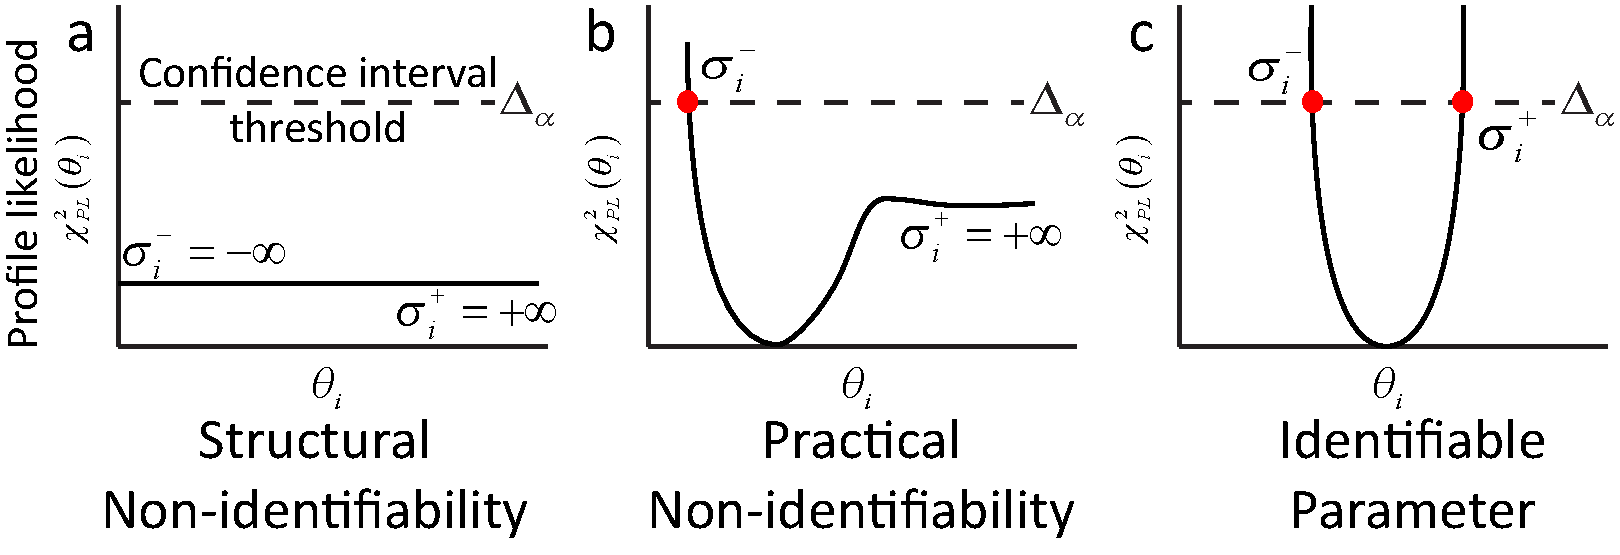
\includegraphics[width=.8\textwidth,height=.8\textheight,keepaspectratio]{figures/identifiability}}
	\caption{The profile likelihood estimates of a) a structurally non-identifiable, b) a practically non-identifiable and c) an identifiable parameter. The horizontal axis represents the changes in the value of the parameter ($\theta_i$) whose identifiability is being determined and the profile likelihood ($\chi^2_{PL}(\theta_i)$) is shown in the vertical axis. The confidence interval threshold ($\Delta_{\alpha}$) used to determine the identifiability of the parameter is denoted by the horizontal dotted line. Identifiable parameters are distinguished from non-identifiable parameters by the presence of both upper and lower bounds on their confidence interval estimates $\left[\sigma_{i}^-,\sigma_{i}^+\right]$. }\label{fig:identtypes}
\end{figure}	

Due to the dependence of practical parameter identifiability on the experimental data, the profile likelihood approach can be used to design experiments in such a way that the observables that are derived from these experiments can improve the practical identifiability of the parameters. We show how experimental design can have a meaningful impact on parameter identification and estimation in Figure \ref{fig:edwithpl}.	Assuming a parameter $\theta_i$ is practically non-identifiable (Figure \ref{fig:edwithpl}a), performing a profile-likelihood based identifiability analysis using simulated data can help determine the nature of experiments needed to make the parameter identifiable (Figure \ref{fig:edwithpl}b). In contrast, performing non-informative experiments without prior knowledge on their ability to change the identifiability of the parameter may provide data that cannot be used to estimate parameter $\theta_i$ (Figure \ref{fig:edwithpl}c).	

%Thus, the identifiability of parameters in nonlinear models is dependent on the model structure, parameterization, and the quality and quantity of experimental data that is available for the purpose of estimation. 